\documentclass[a4paper,10pt]{article}
\usepackage{fullpage}
\usepackage{graphicx}
\usepackage{hyperref}
\usepackage{caption,subcaption}

\begin{document}
\title{\textbf{Rock Paper Scissor}}
\author{
	Alessandro Capici 494022\\
}
\maketitle
\section{The data}
\subsection{Introduction}
Rock Paper Scissors is a two-players game in which each player simultaneously forms one of three shapes with an outstretched hand.\\
A data set has been collected by taking 2188 samples of the three forms. It is divided into a training (1888), a validation (150) and a test (150) set.
\subsection{Samples}
\begin{figure}[h!]
    \centering
    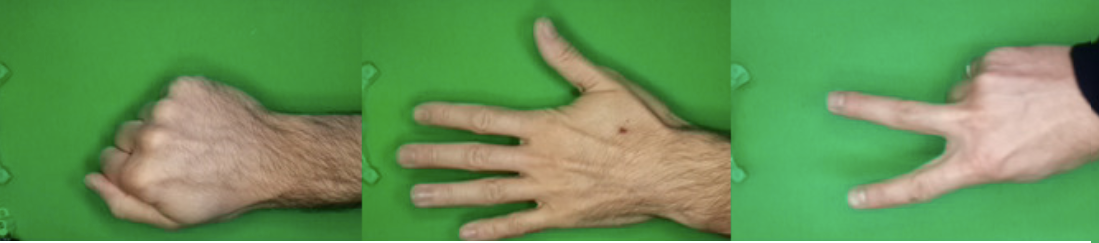
\includegraphics[scale=0.17]{img/0.png}
    \caption{Example of images.}
\end{figure}
Taking a look at the samples we can see that all the images represent a hand in all 3 forms (rock, paper, scissors) resting on a green surface. All the images were captured always following the same hand position, all hands are oriented horizontally with respect to the x axis of the photo and in all photos the fingers are oriented to the left as we can see in the Figure 1. \\
This could be a good indicator on the use of low level features of the type of edge direction, because in this particular case we do not run into problems of rotation and translation, however some images are not perfectly centered with the table frame and this could cause some problems. As for all those low-lever features concerning colors, it is difficult to imagine that their use is fundamental to discriminate the various shapes since many images have different degrees of illumination and in addition there are only 2 colors, the green background and the hand color.
\section{Preprocessing}
Per rendere l immagine adatta ad essere processata da un qualsiasi modello , una proceddura di preprocessing deve essere effettuata, andremo a vederne 2 tipologie.
\subsection{Low Level Feature}
In termini di low level feature per quanto detto precedentemente riguardo alla struttura delle foto andremo ad analizzare due coppie diverse di low level feature:\\
- color based \\
- direction based\\
Comparando i risultati in test e train ottenuti da una semplice rete neurale avente come input la dimensioni della foto e in uscita 3 come le classi i risultati ottenuti sono stati i seguenti:\\
color hist 57.9 /57.3\\
rgb coooc mat 59.6/ 52\\
edge dir hist 71 /68\\
cooc mat 59 / 56\\
Alla luce di questi riusltati combino le la migliore llf per ogni categoria.  In particolare color histogram e edge dir histogram\\ con un risultato finale di 76/74 invece con mean e std 99/94
A questo punto provo a testare qualche metodo di regolarizzazione sui dati per vedere qual è il migliore sulla coppia di feature prima selezionata cioè color hist e edge dir hist
cunando una regolarizzazione sui dati invece sono stati provati 3 tipi di regolarizzzazioni\\
l1 45-46\\
l2 74.8-74\\
mean e std \\99.6-96.6
La normalizzazione con media e std sembra essere quella che da risultati migliori
\subsection{AlexNet}
\section{Model}


color hist + edge dir 128,128 99.9/97.3
\section{Conclusion}
\end{document}